\chapter*{Introduction}\addcontentsline{toc}{chapter}{Introduction}

\section*{Origines de la mécanique quantique}
A la fin du XIXe siècle, les diverses branches de la physique s'intégraient dans un édifice cohérent, basé sur l'étude de deux types d’objets distincts, la matière et le rayonnement:
\begin{itemize}
	\item La matière est faite de corpuscules parfaitement localisables dont le mouvement peut être décrit par la mécanique de Newton. Les grandeurs physiques associées à ces corpuscules s’expriment en fonction des composantes de la position et de l’impulsion qui sont les variables dynamiques fondamentales.
	\item Le rayonnement est gouverné par les lois de l'électromagnétisme de Maxwell. Ses variables dynamiques sont les composantes en chaque point de l’espace des champs électrique et magnétique.
\end{itemize}
Le succès de la physique était à cette époque impressionnant et tous les phénomènes connus trouvaient leur explication dans le cadre de ce programme classique.\\\\

A l’aube du XXe siècle et avec l’essor des progrès technologiques, les physiciens se trouvèrent tout à coup confrontés à des phénomènes nouveaux pour lesquels les prévisions de la théorie classique sont en désaccord flagrant avec l'expérience. Il fallait donc jeter les bases d’une nouvelle théorie susceptible de pallier les insuffisances de la conception classique.

\section*{Contrôle optimal et optimisation numérique}
L'objet de notre étude est un système quantique, modélisé entre deux mesures par l'équation de Schrödinger:
\begin{equation} \label{schrodinger}
i \hbar \dfrac{\partial }{\partial t} \psi (x,t) = H\psi (x,t)
\end{equation}
En vue de modéliser les interactions onde-matière à l'échelle atomique, nous introduisons un contrôle, généré par un dipôle électrostatique de moment dipolaire $\mu (x)$, émettant un champs (électrique) laser, d'amplitude $\varepsilon (t)$ dépendant du temps.\\
La dynamique du système est désormais donnée par:
\begin{equation} \label{eq1}
\begin{cases}
i \hbar \dfrac{\partial }{\partial t} \psi (x,t) &= H\psi (x,t)-\mu(x)\varepsilon(t)\psi (x,t) \\
\psi (x,t=0) &= \psi_0(x)
\end{cases}
\end{equation}
$H$ étant un opérateur hermitien, défini par:
$$
H = H_0 + V = -\dfrac{1}{2m} \varDelta + V
$$
En posant:
\begin{equation}
A(\psi(t),\varepsilon(t))= -i(H-\mu(x)\varepsilon(t))\psi (x,t)
\end{equation}
On se ramène au problème de Cauchy
\begin{equation} \label{chauchy1}
\begin{cases}
\dot{\psi}(t) &= A(\psi(t),\varepsilon(t))\\
\psi (t=0) &= \psi_0
\end{cases}
\end{equation}
Nous nous posons maintenant deux questions.
\subsection*{Problème de contrôlabilité}
Un système est dit contrôlable si on peut le ramener à tout état prédéfini au moyen d’un contrôle. Plus précisément on pose la définition suivante.
\begin{dfn}
On dit que le système \eqref{chauchy1} est contrôlable (ou commandable) si pour tous les états $\psi_0 \in \mathcal{H}$ , $\psi_{cible} \in \mathcal{H}$ , il existe un temps fini $T$ et un contrôle admissible $\varepsilon(.) : [0, T] \longrightarrow \R$ tel que $\psi_{cible} = \psi(T, \psi_0, \varepsilon(.))$.
\end{dfn}
\begin{figure}[H]
	\caption{Problème de contrôlabilité}
	\centering
	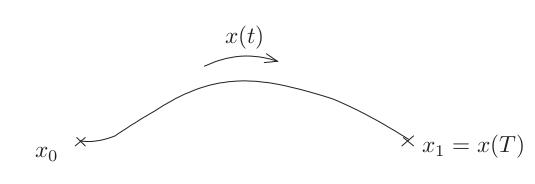
\includegraphics[scale=0.6]{images/controle.png}
\end{figure}
Si la condition précédente est remplie, existe-t-il un contrôle joignant $\psi_0$ à $\psi_{cible}$ , et qui de plus minimise une certaine fonctionnelle $J(\varepsilon)$ ?
\subsection*{Contrôle optimal}
La fonctionnelle $J(\varepsilon)$ est un critère d’optimisation, on l’appelle le coût . Par exemple ce coût
peut être égal au temps de parcours; dans ce cas c’est le problème du temps minimal.
%Nous voulons construire un contrôle d'amplitude "raisonnable" afin d’amener le système d'un état initial $\psi_0$ à un état cible $O\psi(T)$. 
%$O$ étant l'observable décrivant l'état cible. \\\\
\begin{figure}[H]
	\caption{Problème de contrôle optimal}
	\centering
	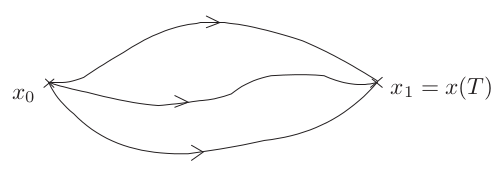
\includegraphics[scale=0.6]{images/controleoptimal.png}
\end{figure}

On considère ainsi une fonctionnelle $J$
\begin{equation}
J(\varepsilon) = \langle \psi(T)|O|\psi(T) \rangle - \alpha \int_{0}^{T}\varepsilon^2(t)dt \quad \alpha \in \R_+
\end{equation}
et on se pose le problème: Trouver $\varepsilon$ tel que $\varepsilon$ résout
$$ \max_{\varepsilon \in L^2(0,T)} J(\varepsilon)$$
Au maximum de la fonctionnelle $J(\varepsilon)$, les équations de Euler-Lagrange sont satisfaites. Le Lagrangien du système est donné par :
\begin{equation} \label{lagrangien}
L(\psi,\varepsilon,\chi)= J(\varepsilon)\\
-2\Re \bigg\{ \int_{0}^{T}\langle \chi (t)|\partial_{t}+i(H_0+V-\mu(x)\varepsilon(t))|\psi(t) \rangle dt \bigg\}
\end{equation}
\section*{Schémas monotones}
Une stratégie éfficace de résolution de ces équations est donnée par une classe d’algorithmes relevant du contrôle quantique, les schémas monotones. Ils ont étés introduits en 1992 par David Tannor, Vladimir Kazakov et V. Orlov,  \cite{Tannor}, sur la base des travaux de Krotov \cite{Krotov1}, \cite{Krotov2}. Une amélioration a ensuite été proposée par Wusheng Zhu et Herschel Rabitz \cite{Zhu} en 1998. Une généralisation est donnée par Yvon Maday et Gabriel Turinici en 2003 \cite{Maday}.\\\\

Comment construire une discrétisation temporelle puis spaciale de ces algorithmes qui préserve la propriété de monotonie?\\\\

Dans le Chapitre Premier, nous introduisons la mécanique quantique en trois postulats et présentons le cadre général du contrôle quantique. Le Chapitre Deux est dédié aux schémas monotones pour l'équation de Schrödinger.
Différentes discrétisations de ces schémas sont proposées dans le Chapitre Trois.